\documentclass[border=4pt]{standalone}
\usepackage{tikz}
\usetikzlibrary{arrows.meta,shapes.geometric}
\begin{document}
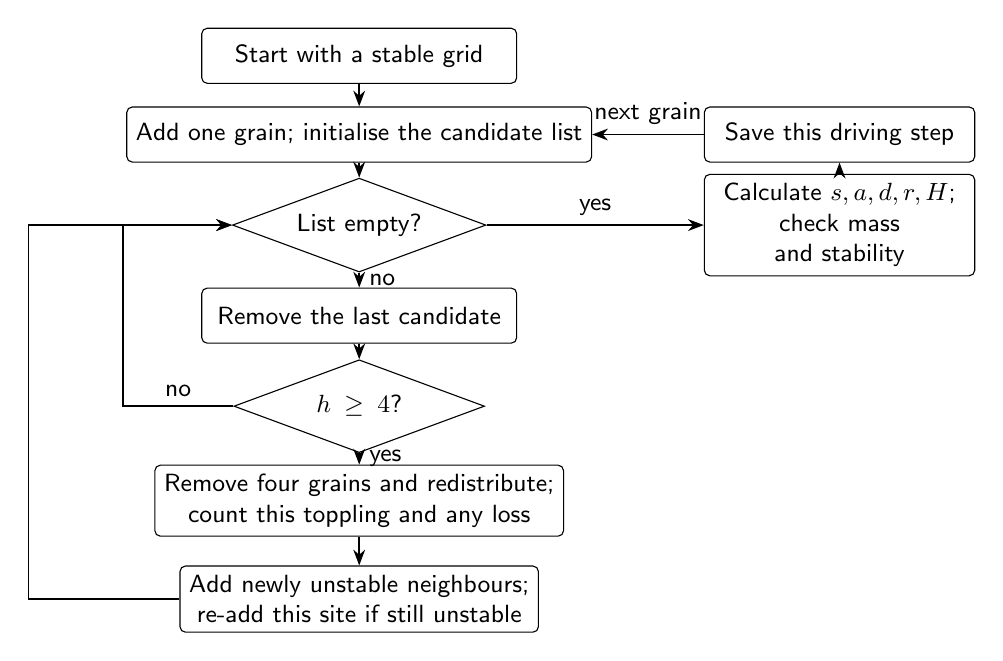
\begin{tikzpicture}[font=\sffamily\small,>=Stealth,
 process/.style={draw,rounded corners=2pt,align=center,minimum width=4cm,minimum height=7mm},
 decision/.style={draw,diamond,aspect=2.7,align=center,inner sep=1pt,text width=2.2cm},
 line/.style={->,line width=.6pt}]
\node[process] (start) at (0,0) {Start with a stable grid};
\node[process] (add) at (0,-1) {Add one grain; initialise the candidate list};
\node[decision] (empty) at (0,-2.15) {List empty?};
\node[process] (pop) at (0,-3.3) {Remove the last candidate};
\node[decision] (unstable) at (0,-4.45) {$h\geq4$?};
\node[process] (topple) at (0,-5.65) {Remove four grains and redistribute;\\count this toppling and any loss};
\node[process] (queue) at (0,-6.9) {Add newly unstable neighbours;\\re-add this site if still unstable};
\node[process,minimum width=3.2cm,text width=3.2cm] (record) at (6.1,-2.15) {Calculate $s,a,d,r,H$;\\check mass and stability};
\node[process,minimum width=3.2cm,text width=3.2cm] (save) at (6.1,-1) {Save this driving step};
\draw[line] (start)--(add);\draw[line] (add)--(empty);
\draw[line] (empty)--node[right]{no}(pop);
\draw[line] (pop)--(unstable);
\draw[line] (unstable)--node[right]{yes}(topple);
\draw[line] (topple)--(queue);
\draw[line] (empty)--node[above]{yes}(record);
\draw[line] (record)--(save);
\draw[line] (save)--node[above]{next grain}(add);
\draw[line] (unstable.west)--node[above]{no}(-3.0,-4.45)--(-3.0,-2.15)--(empty.west);
\draw[line] (queue.west)--(-4.2,-6.9)--(-4.2,-2.15)--(empty.west);
\end{tikzpicture}
\end{document}
